\documentclass[10pt]{report}
\usepackage[letterpaper, margin=0.7in]{geometry}
\usepackage{fontspec}
\usepackage{xcolor}
\usepackage[parfill]{parskip}
\setmainfont{Latin Modern Roman}
\usepackage{graphicx}
\graphicspath{ {./images/} }
\begin{document}

\setcounter{chapter}{5}
\chapter{Data Framing}

\setcounter{section}{1}
\setcounter{subsection}{2}
\subsection{Assignment of Mini Header} \label{mini-header}

\begin{table}[h]
  \begin{tabular}{|p{0.07\linewidth}|c|p{0.15\linewidth}|p{0.5\linewidth}|}
    \hline
    Header Number & x Range & Use & Additional Info \\
    \hline
    \hline
    0x &        & Reserved & \\ \hline
    1x &        & Reserved & \\ \hline
    2x &        & Reserved & \\ \hline
    
    3x & 1 to 5 & Slow Data & Used for character transfer of user's
    data communication via PC.  Data communication of D-PRS is treated
    as slow data communication.  (Range indicates the number of valid
    characters per block.) \\ \hline

    4x & 0 to 3 & Message & Used for messages handled by radio unit's
    display.  (Range indicates indicates the data block number.) \\

    5x & 1 to 5 & Wireless Header Retransmission & Used to retransmit
    the wireless header. \\ \hline

    6x &        & Reserved & (Excluding x = 6) \\ \hline
    66 &        & No Data  & Indicates no data in data frame. \\ \hline
    7x &        & Reserved & \\ \hline
    
    8x & 1 to F & Fast Data & Used for Fast Data transmission.  Range
    indicates length of data, from 1 to 15 bytes. \\ \hline
    
    9x & 0 to C & Fast Data & Used for Fast Data transmission.  Range
    indicates length of data, from 16 to 28 bytes. \\ \hline

    Ax &        & Reserved & \\ \hline
    Bx &        & Reserved & \\ \hline

    Cx & 2      & Code Squelch & Data indicates two-digit code of code
    squelch. \\ \hline

    Dx &        & Reserved & \\ \hline
    Ex &        & Reserved & \\ \hline
    Fx &        & Reserved & \\ \hline
  \end{tabular}
\end{table}

\setcounter{chapter}{6}
\chapter{Fast Data}

Follow this definition to use voice frames for data.  Normal voice
frames should be used when PTT is pressed.

\section{Fast Data Frame Structure}

Fast Data follows the same format of slow data, except the handling of
audio frames and mini header assignments are different (see Chapter
6).

Block number 1 includes the sync frame and is longer than blocks 2-10.
If it is necessary to switch to audio, wait for the end of the current
Fast Data block boundary before starting a normal slow data block with
voice data.

Note: The beep tone should be included during a Fast Data transmission
about every 1 second.  The slow data block with a beep tone should be
inserted between Fast Data block boundaries.

This data transfer method has a speed of about 3480bps.

\section{Fast Data Block Layout}

Note: The images below use the term ``Pin header'' to refer to the
mini header discussed in Section \ref{mini-header}.

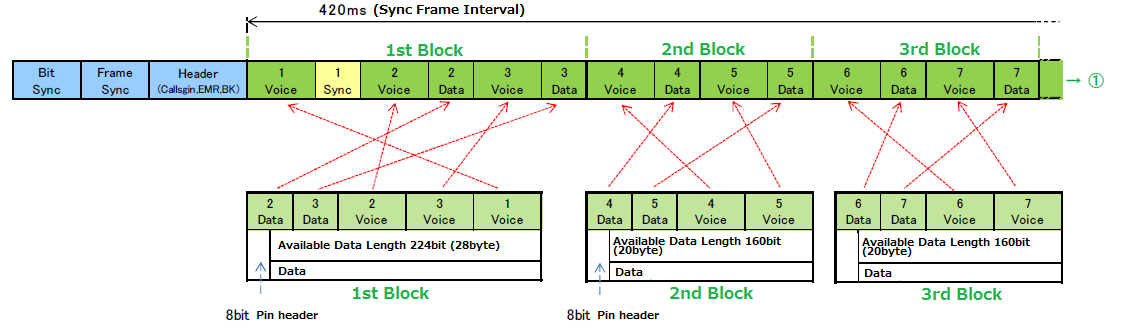
\includegraphics[scale=0.6]{1-3} \\
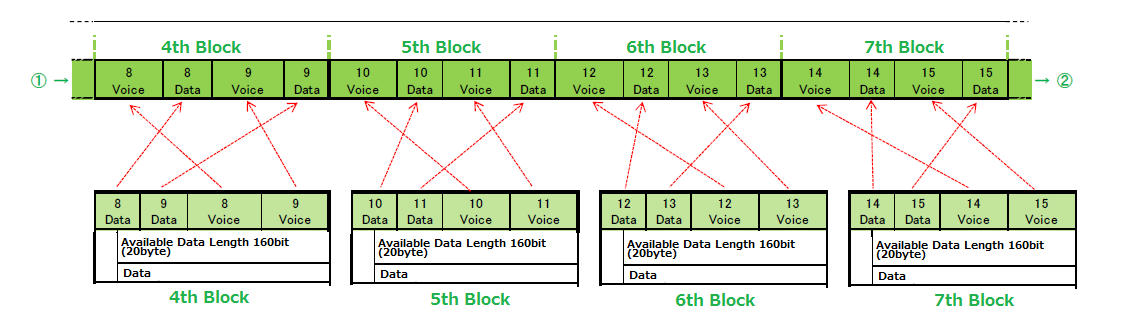
\includegraphics[scale=0.6]{4-7} \\
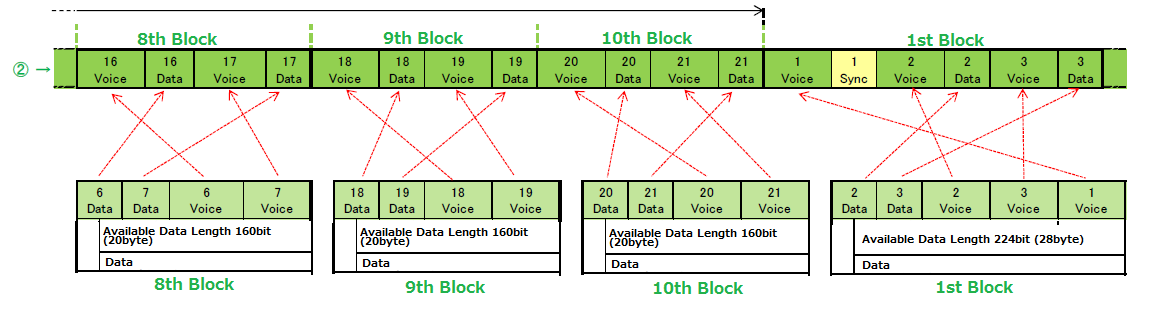
\includegraphics[scale=0.6]{8-10}

\section{Block Assembly of Fast Data}

Only the block containing Sync (block number 1) has an effective data
length of 28 bytes (224 bits):

\small{}
\begin{tabular}{|c|c|c|c|c|c|c|c|c|c|c|c|c|c|}
  \hline
  \multicolumn{13}{|c|}{\textbf{Fast Data, Block 1}} \\
  \hline
  \multicolumn{2}{|c|}{2nd Data} &
  \multicolumn{2}{|c|}{3rd Data} &
  \multicolumn{3}{|c|}{2nd Voice} &
  \multicolumn{3}{|c|}{3rd Voice} &
  \multicolumn{3}{|c|}{1st Voice} \\
  \hline
  \multicolumn{4}{|c|}{4 bytes of effective data} &
  \multicolumn{9}{|c|}{24 bytes of effective data} \\
  \hline
  1 byte & 2 bytes &
  1 byte & 2 bytes &
  4 bytes & 1 byte & 4 bytes &
  4 bytes & 1 byte & 4 bytes &
  4 bytes & 1 byte & 4 bytes \\
  \hline
  Header & \textcolor{teal}{Data} &
  \textcolor{red}{Guard} & \textcolor{teal}{Data} &
  \textcolor{teal}{Data} & \textcolor{red}{N.R.} & \textcolor{teal}{Data} &
  \textcolor{teal}{Data} & \textcolor{red}{N.R.} & \textcolor{teal}{Data} &
  \textcolor{teal}{Data} & \textcolor{red}{N.R.} & \textcolor{teal}{Data} \\
  \hline
\end{tabular}
\normalsize{}

Blocks that do not contain Sync (block numbers 2 to 10) have an
effective data length of 20 bytes (160 bits):

\small{}
\begin{tabular}{|c|c|c|c|c|c|c|c|c|c|c|}
  \hline
  \multicolumn{10}{|c|}{\textbf{Fast Data, Blocks 2-10 (labeled as Block 2)}} \\
  \hline
  \multicolumn{2}{|c|}{4th Data} &
  \multicolumn{2}{|c|}{5th Data} &
  \multicolumn{3}{|c|}{4th Voice} &
  \multicolumn{3}{|c|}{5th Voice} \\
  \hline
  \multicolumn{4}{|c|}{4 bytes of effective data} &
  \multicolumn{6}{|c|}{16 bytes of effective data} \\
  \hline
  1 byte & 2 bytes &
  1 byte & 2 bytes &
  4 bytes & 1 byte & 4 bytes &
  4 bytes & 1 byte & 4 bytes \\
  \hline
  Header & \textcolor{teal}{Data} &
  \textcolor{red}{Guard} & \textcolor{teal}{Data} &
  \textcolor{teal}{Data} & \textcolor{red}{N.R.} & \textcolor{teal}{Data} &
  \textcolor{teal}{Data} & \textcolor{red}{N.R.} & \textcolor{teal}{Data} \\
  \hline
\end{tabular}
\normalsize{}

\small{}
\begin{description}
\item[Header] Mini-header byte as described in Section \ref{mini-header}.
\item[Guard] A guard bit to prevent false detection of packet loss,
  an arbitrary value not matching the packet loss pattern is
  adopted.
\item[N.R. (Noise reduction)] Always assign 0x02 with a bit to
  reduce abnormal noise of the vocoder on the receiving side when
  receiving on an existing model
\end{description}
\normalsize{}

\section{Fast Data Scrambling}

Scrambling is applied to the Fast Data voice and data frames according
to the specification in Appendix 1.

(See images in original STD5\_0b.pdf from JARL)

\end{document}
